\documentclass[11pt,a4paper,oneside]{report}

\usepackage[T1]{fontenc}
\usepackage[utf8]{inputenc}
\usepackage[italian]{babel}
\usepackage[a4paper,margin=2.8cm,top=3cm,bottom=3cm]{geometry}
\usepackage{amsmath,amssymb}
\usepackage{mathpazo}
\usepackage{xcolor}
\usepackage{titlesec}
\usepackage{booktabs}
\usepackage{longtable}
\usepackage{array}
\usepackage{enumitem}
\usepackage{fancyhdr}
\usepackage{graphicx}
\usepackage{tikz}
\usepackage{listings}
\usepackage[most]{tcolorbox}
\usepackage[hidelinks]{hyperref}

\usetikzlibrary{arrows.meta,positioning,fit,backgrounds,calc}

\definecolor{accent}{HTML}{1F3A5F}
\definecolor{soft}{HTML}{6B7C93}
\definecolor{rule}{HTML}{C8D0DA}
\definecolor{boxbg}{HTML}{F4F6F9}
\definecolor{good}{HTML}{2E7D52}
\definecolor{bad}{HTML}{A33A3A}
\definecolor{codebg}{HTML}{F7F8FA}

\hypersetup{colorlinks=true,linkcolor=accent,urlcolor=accent,citecolor=accent}

\titleformat{\chapter}[display]
  {\normalfont\Large\bfseries\color{accent}}
  {\normalfont\normalsize\color{soft}\MakeUppercase{\chaptertitlename}\ \thechapter}
  {0.6em}{\Huge}
\titlespacing*{\chapter}{0pt}{-10pt}{30pt}
\titleformat{\section}{\normalfont\large\bfseries\color{accent}}{\thesection}{0.6em}{}
\titleformat{\subsection}{\normalfont\normalsize\bfseries\color{accent}}{\thesubsection}{0.6em}{}

\pagestyle{fancy}
\fancyhf{}
\renewcommand{\headrulewidth}{0.4pt}
\fancyhead[L]{\small\color{soft}\nouppercase{\leftmark}}
\fancyhead[R]{\small\color{soft}\thepage}

\setlist[itemize]{leftmargin=1.3em,itemsep=2pt,topsep=4pt}
\setlist[enumerate]{leftmargin=1.5em,itemsep=2pt,topsep=4pt}

\lstset{
  basicstyle=\ttfamily\footnotesize,
  backgroundcolor=\color{codebg},
  frame=none,
  breaklines=true,
  columns=fullflexible,
  keepspaces=true,
  xleftmargin=8pt,
  framexleftmargin=8pt,
  aboveskip=8pt, belowskip=8pt,
}

\newtcolorbox{prima}[1][]{colback=boxbg,colframe=rule,boxrule=0.5pt,
  arc=2pt,left=8pt,right=8pt,top=6pt,bottom=6pt,
  title={\color{accent}\bfseries #1},coltitle=accent,
  fonttitle=\bfseries,colbacktitle=boxbg,titlerule=0pt}

\newtcolorbox{lezione}{colback=white,colframe=accent,boxrule=1pt,
  arc=2pt,left=10pt,right=10pt,top=7pt,bottom=7pt,
  borderline west={3pt}{0pt}{accent}}

\newcommand{\tick}{\textcolor{good}{\textbf{\checkmark}}}
\newcommand{\cross}{\textcolor{bad}{\textbf{\texttimes}}}

\begin{document}

\begin{titlepage}
\centering
\vspace*{3cm}
{\color{soft}\large Quaderno di lavoro}\\[1.2cm]
{\color{accent}\Huge\bfseries Che cosa è cambiato\\[0.3cm] e perché}\\[0.9cm]
{\Large Settembre 2026 --- dal laboratorio emulato\\ al datapath reale}\\[2.5cm]
\rule{0.6\linewidth}{0.8pt}\\[0.8cm]
{\large Progetto \textbf{IPA/eBPF}}\\[0.3cm]
{\color{soft} inferenza di una rete neurale dentro il kernel, a bordo del pacchetto}
\vfill
{\color{soft}\small Ogni numero di questo quaderno viene da una misura eseguita,\\
non da una stima. Dove una cosa non è stata verificata, è scritto.}
\end{titlepage}

\tableofcontents
\clearpage

% ==================================================================
\chapter{Di che cosa stiamo parlando}

\section{L'idea in una pagina}

Un router normale decide dove mandare un pacchetto consultando una tabella
riempita da un protocollo di routing. L'idea di \textbf{IPA} (\emph{Intelligent
PAckets}) è diversa: il pacchetto \textbf{porta con sé} una piccola rete
neurale, e ogni nodo che attraversa la esegue per decidere l'uscita.

Niente segnalazione, niente tabella condivisa: la decisione nasce dai dati che
il nodo ha sotto mano in quel momento.

\begin{center}
\begin{tikzpicture}[
  node distance=8mm,
  box/.style={draw=rule,fill=boxbg,rounded corners=2pt,minimum height=8mm,
              inner sep=5pt,font=\small},
  arr/.style={-{Stealth[length=5pt]},draw=soft,thick}
]
\node[box] (p) {pacchetto};
\node[box,right=14mm of p] (n) {nodo};
\node[box,below=9mm of n,fill=white] (st) {stato locale del nodo};
\node[box,right=14mm of n] (o) {porta di uscita};
\draw[arr] (p) -- (n);
\draw[arr] (st) -- (n);
\draw[arr] (n) -- (o);
\node[font=\scriptsize\itshape,color=soft,above=1mm of p] {pesi + descrittore};
\node[font=\scriptsize\itshape,color=soft,below=1mm of st]
     {link su/giù, TTL, interfaccia d'ingresso};
\end{tikzpicture}
\end{center}

Il modello è una rete piccola: quattro tipi di ingresso, due strati nascosti da
quattro neuroni, sette uscite. In tutto \textbf{319 pesi}. Deve stare in un
header ed essere eseguibile in decine di nanosecondi.

\section{Dove gira: XDP}

Il codice gira in \textbf{eBPF} agganciato a \textbf{XDP}, il punto più
precoce in cui il kernel Linux permette di toccare un pacchetto: prima che
venga costruita la struttura \texttt{sk\_buff}, quindi prima di quasi tutto il
resto dello stack di rete.

Questo impone un vincolo forte, che spiega metà delle scelte di progetto: un
programma eBPF deve essere \textbf{dimostrato sicuro} da un componente del
kernel chiamato \emph{verificatore} prima di poter girare. Niente cicli di
lunghezza ignota, niente accessi non controllati alla memoria, niente
ricorsione. Tutto ciò che nel documento sembra contorto — cicli srotolati,
tetti dichiarati a priori, tabelle al posto di calcoli — nasce da lì.

\section{Le tre pipeline}

Lo stesso modello è implementato in tre modi, per misurare un compromesso.

\begin{center}
\small
\begin{tabular}{@{}lll@{}}
\toprule
& \textbf{i pesi stanno} & \textbf{cambiare modello} \\
\midrule
\textbf{P1} hardcoded & scritti nel codice C & ricompilare \\
\textbf{P2} template  & in una mappa         & scrivere la mappa \\
\textbf{P3} modular   & in una mappa, uno strato per programma & scrivere la mappa \\
\bottomrule
\end{tabular}
\end{center}

P1 è veloce perché il compilatore vede i pesi e li semplifica; è rigido perché
ogni modello nuovo richiede una ricompilazione. P2 e P3 sono l'opposto. Il
lavoro di settembre serve a rendere questo confronto \emph{misurabile davvero}.

% ==================================================================
\chapter{La matematica che sta dentro il kernel}

\section{Perché i numeri sono interi}

Nel kernel non ci sono numeri in virgola mobile: eBPF lavora con interi. Il
modello però è addestrato in virgola mobile. Serve una conversione, e si chiama
\textbf{quantizzazione}.

Ogni peso reale $w$ diventa un intero a 8 bit:
\[
  w_{\text{int}} = \operatorname{round}(w \cdot s)
\]
dove $s$ è il \textbf{fattore di scala}, uno solo per tutta la rete.

Perché il risultato stia in un byte con segno serve
\[
  s \cdot \max_i |w_i| \;\le\; 127 .
\]

Sul modello depositato $\max|w| = 5{,}098$, quindi $s \le 24{,}9$. Due scelte
convivono nel progetto: $s = 24$ (il massimo intero ammesso) e $s = 16$ (la
potenza di due più vicina per difetto, che rende le divisioni degli shift).

\begin{lezione}
Superare quel limite non dà un errore: dà un \emph{overflow silenzioso}. I pesi
grandi si troncano e il modello sbaglia senza che nulla lo segnali. Per questo i
test distinguono le scale \emph{rappresentabili} da quelle che saturano, e
misurano solo sulle prime.
\end{lezione}

\section{Il problema dei bias, e l'errore che ci stava dentro}

Qui sta l'errore più sottile trovato in settembre, e vale la pena seguirlo
passo passo perché è istruttivo.

Quando moltiplichiamo un ingresso per un peso quantizzato, il risultato porta
un fattore $s$ in più rispetto al valore reale:
\[
  x \cdot w_{\text{int}} \;=\; x \cdot w \cdot s .
\]

Se impiliamo gli strati, quel fattore si accumula. Dopo $\ell+1$ moltiplicazioni
l'accumulatore dello strato $\ell$ porta $s^{\ell+1}$.

Ma il \textbf{bias} è memorizzato come un peso qualsiasi, cioè con un solo
fattore $s$. Sommarlo così com'è significa sommare una quantità
sistematicamente troppo piccola. Va riportato nelle unità dell'accumulatore:

\begin{center}
\begin{tikzpicture}[
  lay/.style={draw=rule,fill=boxbg,rounded corners=2pt,minimum width=30mm,
              minimum height=9mm,font=\small},
  arr/.style={-{Stealth[length=5pt]},draw=soft,thick}
]
\node[lay] (l0) {strato 0};
\node[lay,right=16mm of l0] (l1) {strato 1};
\node[lay,right=16mm of l1] (l2) {uscita};
\draw[arr] (l0) -- (l1);
\draw[arr] (l1) -- (l2);
\node[font=\scriptsize,color=soft,below=2mm of l0] {accumulatore $s^1$};
\node[font=\scriptsize,color=soft,below=2mm of l1] {accumulatore $s^2$};
\node[font=\scriptsize,color=soft,below=2mm of l2] {accumulatore $s^3$};
\node[font=\scriptsize,color=accent,above=2mm of l0] {bias $\times\, s^0$};
\node[font=\scriptsize,color=accent,above=2mm of l1] {bias $\times\, s^1$};
\node[font=\scriptsize,color=accent,above=2mm of l2] {bias $\times\, s^2$};
\end{tikzpicture}
\end{center}

La regola è semplice: allo strato $\ell$ (contando da zero) il bias va
moltiplicato per $s^{\ell}$.

\begin{prima}[L'errore]
Il modello di riferimento in Python --- quello con cui si controlla che il
datapath calcoli la cosa giusta --- applicava $s^0$ e $s^1$ correttamente ai
primi due strati, e lasciava l'\textbf{ultimo strato a $s^0$} invece di $s^2$.

Il bias dell'uscita era sottopesato di $s^2 = 24^2 = 576$.
\end{prima}

\begin{prima}[Perché nessuno se n'era accorto per mesi]
Tutti i test eseguivano il modello con \textbf{tutti i link attivi}. In quella
condizione gli accumulatori sono grandi e un errore di 576 non sposta mai il
massimo. Basta spegnere qualche link perché gli accumulatori si riducano e
l'errore decida l'esito.

Nello stesso file c'era una seconda funzione di riferimento, scritta per forme
arbitrarie, che usava la formula generale $s^{\ell}$ ed era \textbf{già
corretta}. Due riferimenti, uno giusto e uno sbagliato, e quello sbagliato era
l'unico mai esercitato con link spenti.
\end{prima}

Corretto l'errore, il riferimento e le tre pipeline concordano su tutti i casi
provati.

\begin{lezione}
La lezione non è "c'era un bug". È che \textbf{un test che varia un solo
ingresso non è un test}: verifica una condizione e la ripete. Ci torneremo nel
capitolo~5, dove lo stesso schema si ripresenta in una forma ancora più netta.
\end{lezione}

\section{Il TTL: dividere il prodotto, mai il valore}

Il modello è addestrato con il TTL \emph{normalizzato}, cioè
$\text{ttl}/T$ con $T = 30$ il valore iniziale. Con i numeri interi
\[
  \frac{\text{ttl}}{30} = 0 \qquad \text{per ogni } \text{ttl} < 30 ,
\]
e la feature sparirebbe. La divisione va quindi applicata al \emph{prodotto}:
\[
  \left\lfloor \frac{\text{ttl} \cdot w_{\text{int}}}{T} \right\rfloor
  \quad\text{e non}\quad
  \left\lfloor \frac{\text{ttl}}{T} \right\rfloor \cdot w_{\text{int}} .
\]

Nel C generato si legge esattamente così:
\begin{lstlisting}
(((__s64)_ttl * 11LL) / 30LL)
\end{lstlisting}

% ==================================================================
\chapter{Le classi non sono porte}

\section{Il problema}

La rete produce sette numeri; il più grande vince. Ma \emph{che cosa significa}
la classe vincente?

All'inizio di settembre la risposta era sparsa e incoerente. In punti diversi
del progetto convivevano quattro convenzioni su quale classe significasse
"scarta il pacchetto":

\begin{center}
\small
\begin{tabular}{@{}ll@{}}
\toprule
\textbf{Convenzione} & \textbf{Dove} \\
\midrule
la classe 6 è DROP & in un punto \\
la classe 5 è DROP & in un altro \\
DROP $=$ $n_{\text{out}} - 1$ & in un terzo \\
DROP $=$ $\max(\text{etichette}) + 1$ & dedotto dai dati \\
\bottomrule
\end{tabular}
\end{center}

E sotto ce n'era una quinta, implicita e più insidiosa: che la classe $k$
volesse dire "manda fuori dall'interfaccia $k$". Funzionava per caso, perché nel
modello depositato le porte sono numerate come le classi.

\section{La soluzione: una catena esplicita}

Adesso il significato è \textbf{dichiarato}, mai dedotto, e passa per una
catena di quattro passi, ognuno con un responsabile diverso:

\begin{center}
\begin{tikzpicture}[
  box/.style={draw=rule,fill=boxbg,rounded corners=2pt,minimum height=9mm,
              inner sep=6pt,font=\small,align=center},
  arr/.style={-{Stealth[length=5pt]},draw=accent,thick}
]
\node[box] (c) {classe\\{\scriptsize il modello}};
\node[box,right=11mm of c] (a) {azione\\{\scriptsize il descrittore}};
\node[box,right=11mm of a] (p) {porta logica\\{\scriptsize il descrittore}};
\node[box,right=11mm of p] (i) {ifindex\\{\scriptsize il nodo}};
\draw[arr] (c) -- (a);
\draw[arr] (a) -- (p);
\draw[arr] (p) -- (i);
\end{tikzpicture}
\end{center}

\begin{itemize}
\item \textbf{classe}: quello che il modello ha calcolato;
\item \textbf{azione}: \texttt{FORWARD}, \texttt{DROP} o \texttt{UNUSED} --- una
      classe mai addestrata esiste ed è dichiarata tale;
\item \textbf{porta logica}: un numero che il \emph{modello} conosce;
\item \textbf{ifindex}: l'interfaccia vera, che solo il \emph{nodo} conosce e
      che è diversa su ogni macchina.
\end{itemize}

Nel modello depositato la dichiarazione è:

\begin{center}
\small
\begin{tabular}{@{}rll@{}}
\toprule
\textbf{classe} & \textbf{azione} & \textbf{porta logica} \\
\midrule
0--4 & FORWARD & 0--4 \\
5    & DROP    & --- \\
6    & UNUSED  & --- \\
\bottomrule
\end{tabular}
\end{center}

\begin{lezione}
Il punto non è che adesso funziona: funzionava anche prima, per coincidenza
numerica. Il punto è che adesso \textbf{smetterebbe di funzionare rumorosamente}
se il modello cambiasse, invece di continuare a girare dando risposte
plausibili e sbagliate.
\end{lezione}

\section{Un errore che questa separazione ha fatto emergere}

Il datapath teneva un contatore per classe, ma scriveva nella casella
della \emph{porta} invece che in quella della \emph{classe}. Sembrava
giusto perché le due numerazioni coincidono nel modello depositato.

Con un modello in cui non coincidono, il contatore avrebbe misurato la cosa
sbagliata in silenzio. Separare i due spazi di indici ha reso l'errore visibile
e correggibile.

% ==================================================================
\chapter{Il motore non è lo scenario}

\section{Com'era}

Il progetto era nato attorno a una topologia precisa: \textbf{Germany50}, una
rete di 50 router usata come riferimento in letteratura, con due host attaccati,
emulata con \textbf{Kathara} (container Docker connessi a formare la rete).

Due numeri erano ovunque nel codice:
\[
  n_{\text{nodi}} = 52, \qquad n_{\text{interfacce}} = 6 .
\]

Il primo è $50 + 2$. Il secondo è il \textbf{grado massimo} della rete: il nodo
con più vicini. Non è il grado di un nodo qualsiasi --- tutti gli altri riempiono
di zeri gli slot che non usano.

Questi numeri determinano la larghezza dell'ingresso:
\[
  n_{\text{in}} = \underbrace{6}_{\text{link}} + \underbrace{6}_{\text{iface}}
  + \underbrace{1}_{\text{ttl}} + \underbrace{52}_{\text{nodo}} = 65 .
\]

Il problema non era che esistessero, ma che il motore li conoscesse. C'era un
\emph{default} interno: se nessuno diceva niente, il motore assumeva 6 e 52.
Ogni chiamante che dimenticava di specificare lo scenario risultava
silenziosamente corretto per Germany50 e silenziosamente sbagliato altrove.

\section{Com'è adesso: tre strati}

\begin{center}
\begin{tikzpicture}[
  lay/.style={draw=rule,fill=boxbg,rounded corners=3pt,minimum width=74mm,
              minimum height=13mm,inner sep=6pt,font=\small,align=left},
  arr/.style={-{Stealth[length=6pt]},draw=accent,very thick}
]
\node[lay] (a) {\textbf{Motore} \\ {\scriptsize pipeline, inferenza, semantica delle classi}};
\node[lay,below=11mm of a] (b) {\textbf{Configurazione} \\ {\scriptsize quanti nodi, quante interfacce, che modello}};
\node[lay,below=11mm of b] (c) {\textbf{Scenario} \\ {\scriptsize la rete concreta su cui si misura}};
\draw[arr] (c) -- node[right,font=\scriptsize\itshape,color=soft] {descrive} (b);
\draw[arr] (b) -- node[right,font=\scriptsize\itshape,color=soft] {configura} (a);
\end{tikzpicture}
\end{center}

La dipendenza punta \textbf{solo verso l'alto}. Il motore non sa che cosa sia
Germany50.

Le dimensioni si risolvono in ordine: una variabile d'ambiente, poi un file di
sistema, poi il blocco \texttt{trained\_on} del descrittore del modello. Se
nessuna delle tre risponde, il motore \textbf{si ferma} e dice dove ha cercato.

\begin{lezione}
Un default comodo è il modo più efficace di nascondere un'assunzione. Preferire
un errore esplicito a un valore plausibile è una scelta di progetto, non
pignoleria: il valore plausibile non si manifesta mai come errore, solo come
risultato sbagliato mesi dopo.
\end{lezione}

\section{La prova}

Non basta dirlo. Il motore genera oggi un datapath corretto per cinque
topologie che non hanno niente a che vedere con quella d'origine:

\begin{center}
\small
\begin{tabular}{@{}rrlrrl@{}}
\toprule
\textbf{iface} & \textbf{nodi} & \textbf{strati} & $n_{\text{in}}$ & $n_{\text{out}}$ & \textbf{vettore link} \\
\midrule
3 &  8 & 4-4     & 15 & 4 & \texttt{v[3]} \\
4 & 16 & 6       & 25 & 5 & \texttt{v[4]} \\
5 & 24 & 4-4-4   & 35 & 6 & \texttt{v[5]} \\
2 &  6 & 3-3     & 11 & 3 & \texttt{v[2]} \\
6 & 52 & 4-4     & 65 & 7 & \texttt{v[6]} \\
\bottomrule
\end{tabular}
\end{center}

Nessuna riga di C scritta a mano cambia fra una riga e l'altra.

% ==================================================================
\chapter{Dall'emulatore al kernel vero}

\section{Che cosa provavano i test di prima}

Fino a settembre ogni misura veniva da una chiamata di sistema,
\mbox{\texttt{BPF\_PROG\_TEST\_RUN}}: si dà al programma un buffer, lo si
esegue $N$ volte, e il kernel riporta quanti nanosecondi in media.

È utile e onesto per confrontare le tre pipeline fra loro. Ma non tocca
un'interfaccia, non ha un driver, non consegna niente. Il programma poteva dire
\emph{"redirigerei sulla porta 3"} e nessuno verificava che un pacchetto ne
uscisse davvero.

\section{Il banco nuovo}

Kathara è stato sostituito da qualcosa di più semplice e più vicino al vero:
coppie di interfacce virtuali (\texttt{veth}) create sull'host.

\begin{center}
\begin{tikzpicture}[
  n/.style={draw=rule,fill=boxbg,rounded corners=2pt,minimum width=17mm,
            minimum height=7mm,font=\scriptsize},
  arr/.style={-{Stealth[length=4pt]},draw=soft},
  xdp/.style={draw=accent,fill=white,rounded corners=2pt,minimum width=22mm,
              minimum height=9mm,font=\scriptsize,thick}
]
\node[n] (inp) {\texttt{ipainp}};
\node[xdp,right=9mm of inp] (ing) {\texttt{ipain} + XDP};
\node[n,right=13mm of ing,yshift=13mm] (p0) {\texttt{ipa0}};
\node[n,right=13mm of ing,yshift=0mm]  (p1) {\texttt{ipa1}};
\node[n,right=13mm of ing,yshift=-13mm](p2) {\texttt{ipa2}};
\node[n,right=8mm of p0] (q0) {\texttt{ipa0p}};
\node[n,right=8mm of p1] (q1) {\texttt{ipa1p}};
\node[n,right=8mm of p2] (q2) {\texttt{ipa2p}};
\draw[arr] (inp) -- (ing);
\draw[arr] (ing) -- (p0);
\draw[arr] (ing) -- (p1);
\draw[arr] (ing) -- (p2);
\draw[arr] (p0) -- (q0);
\draw[arr] (p1) -- (q1);
\draw[arr] (p2) -- (q2);
\node[font=\scriptsize\itshape,color=soft,below=1mm of inp,align=center]
     {iniezione};
\node[font=\scriptsize\itshape,color=soft,right=1mm of q2,align=left]
     {cattura};
\end{tikzpicture}
\end{center}

Si inietta un frame da un capo, il programma XDP gira davvero, e si legge da
quale interfaccia è uscito. Questo risponde alla domanda che
\texttt{BPF\_PROG\_TEST\_RUN} non può porre.

\subsection*{Due dettagli che sembrano minori e non lo sono}

\textbf{Modalità di attacco.} XDP si può agganciare in due modi: \emph{native},
dentro il driver, prima che esista la \texttt{sk\_buff}; oppure \emph{generic},
dopo. Il progetto usava sempre generic, e il motivo era scritto nel codice:
serviva per le interfacce dentro i container dell'emulatore. Tolto l'emulatore,
quel motivo cade. Adesso il default è native, la modalità \emph{davvero in
effetto} viene riletta dal kernel dopo l'aggancio, e un fallimento è un errore,
non una retrocessione silenziosa.

\textbf{Il vincolo delle veth.} Redirigere \emph{verso} una veth funziona solo
se il lato ricevente ha a sua volta un programma XDP agganciato: il kernel
alloca le code necessarie solo in quel caso. Senza, il redirect fallisce in
silenzio e il pacchetto sparisce --- indistinguibile da un modello che decide di
scartare tutto. Il banco aggancia quindi un programma minimo a ogni capo.

\section{Tre difetti del test, trovati misurando}

Il banco nuovo ha trovato più difetti nei \emph{test} che nel prodotto. Vale la
pena elencarli, perché il motivo per cui erano invisibili è sempre lo stesso.

\begin{prima}[1. Il TTL non muove questo modello]
La prima versione del test variava il TTL da 2 a 8 e riportava
\emph{"7 verifiche su 7 superate"}.

Misurando lo spazio raggiungibile si scopre che con tutti i link attivi il
modello risponde \textbf{sempre classe 2}, per qualsiasi TTL. Quel 7 su 7 era
\textbf{un caso solo, ripetuto sette volte}.

È \texttt{link\_state} la feature che sposta la decisione. Il test adesso
\emph{cerca} un ingresso per ogni classe, invece di spazzare alla cieca.
\end{prima}

\begin{prima}[2. Un pacchetto del kernel contato come risultato]
Su una veth appena creata il kernel manda del traffico suo (IPv6 multicast). Una
volta è stato catturato e contato come la risposta della pipeline. È passato per
caso, perché era sulla porta giusta.

Adesso la cattura filtra sui campi che il datapath non riscrive, e IPv6 viene
disabilitato sulle interfacce del banco.
\end{prima}

\begin{prima}[3. La porta 0 era invisibile per costruzione]
L'ingresso era anche la porta logica 0. Una classe che inoltrava su quella porta
rimandava il frame fuori dall'interfaccia da cui era entrato --- dove la cattura
non lo distingue da quello appena iniettato. Una decisione \emph{corretta} sulla
porta 0 non era osservabile.

Il banco ha adesso un ingresso dedicato, separato da tutte le porte.
\end{prima}

\begin{lezione}
Un test che non può fallire non è un test. In tutti e tre i casi il risultato
era verde e privo di contenuto, e in tutti e tre il difetto è emerso solo
mettendo in mezzo un kernel vero.
\end{lezione}

\section{Il risultato}

Tutte e tre le pipeline superano oggi la verifica end-to-end su un datapath
reale: XDP native, redirect vero, pacchetto ripreso sulla porta d'uscita, e
scarto verificato dal \emph{contatore} e non dal silenzio --- perché "non è
arrivato niente" è anche ciò che si osserva quando il redirect si perde.

% ==================================================================
\chapter{La feature che non c'era}

\section{Il sintomo}

Il modello ha quattro ingressi. Uno di questi è \emph{da quale interfaccia è
arrivato il pacchetto}, codificato \emph{one-hot}: un vettore di sei posizioni
con un solo uno.

Il datapath leggeva l'indice dell'interfaccia dato dal kernel --- l'
\texttt{ifindex} --- e lo usava direttamente come posizione nel vettore, con un
controllo di validità:
\[
  1 \le \text{ifindex} \le n_{\text{interfacce}} .
\]

Gli \texttt{ifindex} però li assegna il kernel, in ordine di creazione. Su un
container appena avviato valgono 2, 3, 4. Su una macchina che ha creato qualche
interfaccia virtuale valgono 205, 217, 229.

Il controllo falliva sempre. \textbf{Nessun bit veniva acceso.} Il modello
girava di fatto su tre ingressi invece di quattro.

\begin{center}
\begin{tikzpicture}[
  box/.style={draw=rule,fill=boxbg,rounded corners=2pt,minimum height=8mm,
              inner sep=5pt,font=\scriptsize,align=center},
  arr/.style={-{Stealth[length=4pt]},draw=soft,thick},
  bad/.style={draw=bad,text=bad}
]
\node[box] (k) {ifindex del kernel\\\texttt{205}};
\node[box,right=13mm of k,bad] (t) {$1 \le x \le 6$ ?};
\node[box,right=13mm of t,bad] (z) {one-hot\\tutto zero};
\draw[arr] (k) -- (t);
\draw[arr] (t) -- node[above,font=\scriptsize,color=bad] {no} (z);
\end{tikzpicture}
\end{center}

\section{Perché nessun test lo vedeva}

Perché nessun test controllava che quella feature \emph{contribuisse} qualcosa.
Riferimento e datapath la ignoravano entrambi, quindi \textbf{concordavano} --- e
l'accordo veniva registrato come successo.

Una pipeline aveva in effetti una tabella di traduzione, ma compilata dentro il
programma come $[2,3,4,5,6,7]$: la stessa assunzione, scritta in un altro modo.
Le altre due usavano l'indice grezzo. Le tre pipeline sceglievano quindi
\emph{colonne diverse} per lo stesso pacchetto --- una discrepanza documentata in
un commento e mai risolta.

\section{La correzione}

La traduzione è diventata una \textbf{tabella a runtime}, riempita dal piano di
controllo leggendo le interfacce del nodo:

\begin{center}
\begin{tikzpicture}[
  box/.style={draw=rule,fill=boxbg,rounded corners=2pt,minimum height=8mm,
              inner sep=5pt,font=\scriptsize,align=center},
  arr/.style={-{Stealth[length=4pt]},draw=accent,thick}
]
\node[box] (k) {ifindex\\\texttt{205}};
\node[box,right=12mm of k,draw=accent] (m) {tabella\\\texttt{ingress\_port}};
\node[box,right=12mm of m,draw=good,text=good] (p) {porta logica\\\texttt{1}};
\draw[arr] (k) -- (m);
\draw[arr] (m) -- (p);
\end{tikzpicture}
\end{center}

È il \textbf{simmetrico} della tabella già usata in uscita: là "quale
interfaccia realizza la porta che il modello ha scelto", qui "quale porta è
l'interfaccia da cui il pacchetto è arrivato". Entrambe sono fatti del nodo,
entrambe si risolvono quando il nodo esiste.

\section{La prova che adesso è viva}

Prima e dopo la correzione, gli ingressi che raggiungono ciascuna classe
\textbf{cambiano}:

\begin{center}
\small
\begin{tabular}{@{}rll@{}}
\toprule
\textbf{classe} & \textbf{prima} (feature morta) & \textbf{dopo} (feature viva) \\
\midrule
0 & \texttt{100110}, ttl 27 & \texttt{100111}, ttl 20 \\
1 & \texttt{010000}, ttl 2  & \texttt{010000}, ttl \textbf{14} \\
5 & \texttt{000000}, ttl 2  & \texttt{000000}, ttl \textbf{12} \\
\bottomrule
\end{tabular}
\end{center}

Stesso stato dei link, TTL diverso per ottenere la stessa classe: l'ingresso in
più contribuisce. E il TTL ora sposta la decisione, cosa che prima non faceva.

\section{Il prezzo, misurato}

Una lettura di tabella in più per pacchetto:

\begin{center}
\small
\begin{tabular}{@{}lrr@{}}
\toprule
& \textbf{prima} & \textbf{dopo} \\
\midrule
letture per pacchetto (P1) & 4,0 & 5,0 \\
letture per pacchetto (P3) & 26,0 & 28,0 \\
istruzioni (P1) & 997 & 971 \\
\bottomrule
\end{tabular}
\end{center}

Le istruzioni di P1 \emph{calano}: la tabella ha sostituito un blocco
\texttt{switch} a sei casi, e una lettura costa meno di un salto.

Una lettura in più arriverà poco dopo, per la stessa ragione applicata a un
altro ingresso: è il capitolo che segue. Le cifre finali sono 6,0 letture per
P1 e 29,0 per P3.

% ==================================================================
\chapter{Il nodo non sapeva di essere un nodo}

\section{L'ingresso più grande di tutti}

Dei quattro ingressi del modello, quello che pesa di più è \emph{quale nodo sta
elaborando il pacchetto}. Su Germany50 sono 52 nodi, quindi un vettore one-hot
di 52 posizioni: \textbf{208 dei 319 pesi} della rete, quasi due terzi.

\section{Il sintomo}

Il datapath riempiva quel vettore con il campo \texttt{model\_id} preso
dall'intestazione IPA del pacchetto.

Sono due cose diverse. \texttt{model\_id} dice \emph{quale modello} il pacchetto
chiede di usare; il vettore vuole sapere \emph{quale nodo} lo sta elaborando. E
il \texttt{model\_id} non cambia lungo il percorso: è scritto dal mittente e
viaggia identico fino alla destinazione.

\begin{lezione}
Con un solo modello registrato --- il caso normale --- \textbf{ogni nodo della
rete accendeva la stessa identica posizione}. Due terzi dei pesi della rete non
distinguevano nulla.
\end{lezione}

\begin{center}
\begin{tikzpicture}[
  box/.style={draw=rule,fill=boxbg,rounded corners=2pt,minimum height=8mm,
              inner sep=5pt,font=\scriptsize,align=center},
  arr/.style={-{Stealth[length=4pt]},draw=soft,thick},
  bad/.style={draw=bad,text=bad},
  ok/.style={draw=good,text=good}
]
\node[box] (n1) {nodo 7};
\node[box,below=4mm of n1] (n2) {nodo 23};
\node[box,below=4mm of n2] (n3) {nodo 41};
\node[box,right=16mm of n2,bad] (m) {\texttt{model\_id} $= 0$\\(dal pacchetto)};
\node[box,right=14mm of m,bad] (o) {one-hot\\posizione 0\\\emph{sempre}};
\draw[arr] (n1) -- (m);
\draw[arr] (n2) -- (m);
\draw[arr] (n3) -- (m);
\draw[arr] (m) -- (o);
\end{tikzpicture}
\end{center}

\section{La correzione, e perché una tabella e non un array}

Stessa forma della correzione precedente: una \textbf{tabella letta a runtime},
riempita quando il nodo viene messo in servizio, dalla variabile d'ambiente
\texttt{IPA\_NODE\_ID} o dall'indice del nodo nella topologia.

Un dettaglio che sembra tecnico e non lo è: la tabella è di tipo \emph{hash} e
non \emph{array}. Un array in questo ambiente è preallocato e riempito di zeri,
quindi una lettura riesce \textbf{sempre}: "non configurato" e "sono il nodo 0"
tornerebbero lo stesso valore, indistinguibili. Sarebbe esattamente il difetto
che la tabella serve a togliere. Con un hash, finché nessuno scrive non c'è
voce: il vettore resta spento, ed è la risposta onesta.

Questo errore è stato commesso e corretto: la prima versione usava un array, e
un test su un'architettura alternativa è fallito 5 volte su 5 prima che se ne
capisse il motivo.

\section{Una pipeline ha resistito un giorno}

P1 e P2 hanno accettato la modifica subito. P3 no: il verificatore del kernel ha
\textbf{rifiutato il programma}, dodici configurazioni di fila.

Il motivo è controintuitivo e vale la pena averlo scritto. Il verificatore non
misura quanto è lungo il programma: esplora i \emph{cammini} possibili, e il
numero di stati che deve tenere è il \textbf{prodotto} dei valori indipendenti
che segue dentro un ciclo srotolato, non la loro somma.

\[
  \text{stati} \;\sim\; v_1 \times v_2 \times \dots \times v_k
\]

L'unica versione che caricava era quella in cui l'indice del nodo \emph{non era
un valore indipendente}: \texttt{nodo = model\_id}, cioè lo stesso registro che
il verificatore stava già seguendo. Un valore, non due.

Escluse una a una, ognuna con la sua prova: il tipo di tabella, la sua
dichiarazione, il valore, il tipo del dato, il numero di letture, la larghezza
in bit. Nessuna era la causa.

Quello che ha liberato spazio non toccava il nodo: un \textbf{tetto} di tutt'altra
feature. Il programma teneva in vita otto posizioni per un vettore di occupazione
delle code che il modello depositato \emph{non dichiara nemmeno}. Portato quel
tetto da 8 a 1, il programma ha caricato --- e più piccolo di prima.

\begin{lezione}
Questi limiti sono \textbf{scogliere, non pendenze}. Nello stesso giro, ridurre
\emph{anche} un secondo tetto --- cioè chiedere \emph{meno} --- ha fatto fallire
di nuovo il caricamento. Un tetto qui si cambia e \textbf{si rimisura}; non si
ragiona.
\end{lezione}

\section{La prova che il nodo è vivo}

Stesso programma compilato, due esecuzioni che differiscono solo per la tabella
del nodo:

\begin{center}
\small
\begin{tabular}{@{}ll@{}}
\toprule
\textbf{esecuzione} & \textbf{esito sul pacchetto} \\
\midrule
senza indice di nodo & scartato \\
indice di nodo $= 7$ & non scartato \\
\bottomrule
\end{tabular}
\end{center}

Nient'altro è cambiato fra le due. L'ingresso sposta la decisione.

% ==================================================================
\chapter{Il verificatore non conta le istruzioni}

\section{Due monete diverse}

Il tetto sulle code portato a 1 era una perdita vera: a 1, un modello che
dichiari davvero quella feature viene \emph{rifiutato}. Per recuperarlo serviva
margine di verifica, e il margine è arrivato da una riscrittura che non toglie
niente.

\section{Il ciclo era girato dalla parte sbagliata}

Il primo strato della rete si calcola così: per ogni neurone, si sommano i
contributi di ogni feature dichiarata nel descrittore.

Il codice lo faceva nell'ordine ovvio --- neuroni fuori, feature dentro:

\begin{lstlisting}
per ogni neurone j (8 volte)
    per ogni feature f (4 volte)
        di che tipo e' f?         <- catena a 5 rami
        di che larghezza e' f?    <- controllo per ogni posizione
        accumula
\end{lstlisting}

Ma \emph{di che tipo} e \emph{di che larghezza} è una feature non dipende dal
neurone. Quella catena a cinque rami veniva quindi rivalutata $8 \times 4 = 32$
volte per pacchetto, e il controllo sulla larghezza di un vettore denso
$8 \times 8 = 64$ volte, per ottenere ogni volta la stessa risposta.

Girato al contrario --- feature fuori, neuroni dentro --- diventa:

\begin{lstlisting}
per ogni feature f (4 volte)
    di che tipo e' f?             <- 4 volte, non 32
    di che larghezza e' f?        <- 8 volte, non 64
    per ogni neurone j (8 volte)
        accumula                  <- nessun ramo qui dentro
\end{lstlisting}

\section{Perché il risultato non cambia di un bit}

Cambia solo l'\textbf{ordine in cui i termini vengono sommati}. I termini sono
gli stessi, calcolati allo stesso modo. E la somma fra interi a 64 bit in
complemento a due è associativa e commutativa --- anche in caso di traboccamento,
che si comporta identicamente nei due ordini:
\[
  (a + b) + c \;=\; a + (b + c) .
\]
Ogni accumulatore finisce quindi \textbf{bit per bit identico}. Non "circa
uguale": identico.

\section{Il risultato, che sembra un errore}

\begin{center}
\small
\begin{tabular}{@{}lrr@{}}
\toprule
& \textbf{prima} & \textbf{dopo} \\
\midrule
P2, programma principale & 16\,144 & \textbf{14\,587} \\
P3, primo strato & 6\,417 & \textbf{6\,850} \\
P3, tetto sulle code caricabile & 1 & \textbf{8} \\
\bottomrule
\end{tabular}
\end{center}

\begin{lezione}
P3 è \textbf{cresciuto} di 433 istruzioni ed è diventato molto più economico da
verificare. Prima della riscrittura, col tetto delle code a 8 non caricava
niente; dopo, carica a 10\,207 istruzioni.

Dimensione del programma e complessità di verifica sono \textbf{monete diverse}.
Il verificatore paga i cammini.
\end{lezione}

\section{Un effetto collaterale che vale una riga di tabella}

Contare quante letture di tabella fa un programma per pacchetto richiede di
ricompilarlo con un contatore su ogni punto di lettura. Le versioni strumentate
di P2 e P3 \textbf{sforavano il verificatore}: per questo la riga "letture di
tabella" riportava \emph{n.d.} per entrambe.

Con il margine liberato dalla riscrittura, tutte e due caricano. La misura che
era impossibile è diventata una riga di tabella --- 11 letture per P2, 29 per P3
--- senza che nessuno abbia riscritto il contatore.

% ==================================================================
\chapter{I numeri, e che cosa dicono davvero}

\section{La tabella}

Misure su una macchina virtuale a 4 processori, modello 65-4-4-7, scala 24.

\begin{center}
\small
\begin{tabular}{@{}lrrrr@{}}
\toprule
& \textbf{baseline} & \textbf{P1} & \textbf{P2} & \textbf{P3} \\
\midrule
istruzioni caricate & 155 & 1\,026 & 14\,628 & 12\,031 \\
salti fra programmi & 0 & 1 & 1 & 3 \\
letture di tabella  & 3,0 & 6,0 & 11,0 & 29,0 \\
memoria delle tabelle & 280 B & 2\,356 B & 10\,416 B & 19\,508 B \\
latenza (minimo di 7) & 29 ns & 73 ns & 262 ns & 421 ns \\
\bottomrule
\end{tabular}
\end{center}

Il \emph{baseline} è un programma che analizza il pacchetto e lo rimanda fuori
senza alcuna inferenza: è il pavimento contro cui si legge tutto il resto.

Tutte le colonne vengono dalla \textbf{stessa esecuzione}, sulla stessa
macchina, nello stesso minuto. La riga "letture di tabella" è piena per la prima
volta: fino alla riscrittura del capitolo precedente, per P2 e P3 diceva
\emph{n.d.}

\section{Primo risultato: la dimensione non predice la velocità}

\begin{lezione}
\textbf{P3 ha il 18\% di istruzioni in meno di P2 ed è il 61\% più lento.}

Il motivo sta nelle due righe centrali: tre salti fra programmi invece di uno, e
ventinove letture di tabella per pacchetto invece di undici.
\end{lezione}

Il conteggio delle istruzioni misura quanto è \emph{grande} il programma
caricato, non quanto \emph{lavoro} fa per pacchetto. In questo regime a dominare
sono le letture di memoria e i salti, non l'aritmetica.

\subsection*{Perché P2 è più grande, pur essendo più veloce}

Le due cose hanno la stessa causa: \textbf{P3 non tiene la rete intera in un
programma}.

\begin{center}
\begin{tikzpicture}[
  box/.style={draw=rule,fill=boxbg,rounded corners=2pt,minimum height=7mm,
              inner sep=4pt,font=\scriptsize,align=center},
  arr/.style={-{Stealth[length=4pt]},draw=soft,thick},
  lp/.style={-{Stealth[length=4pt]},draw=accent,thick}
]
\node[box,draw=accent] (p2) {\textbf{P2} --- un programma solo\\[1pt]
  strato 1 \;+\; strato 2 \;+\; uscita\\[1pt]
  \emph{tutti srotolati insieme: 14\,587}};
\node[box,below=7mm of p2,draw=good] (p3a) {\textbf{P3} --- primo strato: 10\,207};
\node[box,below=4mm of p3a,draw=good] (p3b) {strato denso generico: 1\,688\\[1pt]
  \emph{UNA copia, eseguita DUE volte}};
\draw[lp] (p3a) -- (p3b);
\draw[lp] (p3b.east) -- ++(9mm,0) |- node[right,font=\scriptsize,pos=0.25] {salto} (p3b.north east);
\end{tikzpicture}
\end{center}

P3 srotola \textbf{un} solo strato denso generico e ci rientra, con un salto fra
programmi, a ogni passo della rete. Così la \emph{profondità} del modello non
costa dimensione: un modello a quattro strati gira sullo stesso identico binario.
P2 deve srotolarli tutti, perché è un programma solo --- e un modello più
profondo richiede un altro binario.

Quel riuso è esattamente ciò che P3 paga in latenza: ogni rientro è un salto più
le letture che servono a ricostruire il contesto perduto.

\begin{lezione}
La stessa scelta di progetto spiega \emph{entrambi} i numeri: P3 è più piccolo
\textbf{perché} riusa un pezzo, ed è più lento \textbf{perché} riusarlo costa un
salto e delle letture ogni volta.
\end{lezione}

\section{Secondo risultato: quanto valgono le latenze assolute}

Ogni cifra di latenza in tabella è il \textbf{minimo di sette misure}
indipendenti. Guardando come sono distribuite quelle sette, dentro una singola
esecuzione:

\begin{center}
\small
\begin{tabular}{@{}lrrrr@{}}
\toprule
& baseline & P1 & P2 & P3 \\
\midrule
minimo   & 29 ns & 73 ns & 262 ns & 421 ns \\
mediana  & 30 ns & 88 ns & 278 ns & 453 ns \\
massimo  & 32 ns & 99 ns & 327 ns & 476 ns \\
\midrule
dispersione & 10\% & \textbf{36\%} & 25\% & 13\% \\
\bottomrule
\end{tabular}
\end{center}

Il 36\% di P1 è \emph{dentro} una sola esecuzione, sullo stesso binario, in
pochi secondi. Le \textbf{istruzioni sono identiche} fra esecuzioni diverse: sono
deterministiche. Le latenze no.

\begin{lezione}
Su questa macchina virtuale una differenza di latenza sotto il 20\%--30\%
\textbf{non significa nulla}, nemmeno dentro la stessa esecuzione. Valgono i
rapporti fra le colonne, non le cifre.

Ogni valore assoluto va letto come ordine di grandezza su questa VM, mai come
prestazione del sistema.
\end{lezione}

\subsection*{Un caso in cui la regola è servita}

Il tetto sulle code di P3, riportato da 1 a 8, aggiunge \textbf{3\,357
istruzioni} al programma:

\begin{center}
\small
\begin{tabular}{@{}lrr@{}}
\toprule
& \textbf{tetto 1} & \textbf{tetto 8} \\
\midrule
istruzioni (P3) & 8\,674 & 12\,031 \\
letture per pacchetto & 29,0 & 29,0 \\
\textbf{latenza} & \textbf{419 ns} & \textbf{421 ns} \\
\bottomrule
\end{tabular}
\end{center}

Il 39\% di istruzioni in più costa \textbf{2 nanosecondi}, cioè niente, e le
letture non si muovono di una. Il motivo è semplice: il modello depositato non
dichiara la feature delle code, quindi quel ramo del programma \emph{non viene
mai eseguito}. Cresce la dimensione statica; il percorso eseguito è lo stesso.

\begin{lezione}
Una metrica che si sposta del 39\% senza che cambi nulla di ciò che gira
\textbf{non è una misura di costo}. Il numero di istruzioni va letto come
"quanto è grande il binario", mai come "quanto lavora".
\end{lezione}

Questo ha reso necessario rifare la tabella dei risultati: la versione
precedente presentava tre esecuzioni etichettate come ripetizioni, ma venivano
in realtà da \emph{stati diversi del codice}.

\section{Terzo risultato: la genericità ha un costo di verifica}

P2 serve qualsiasi modello che stia sotto certi tetti dichiarati a priori
(numero massimo di neuroni, di ingressi, di feature). È il suo pregio: non
ricompila mai.

Il conto però lo paga il verificatore del kernel, che percorre ogni cammino del
corpo srotolato. Con i tetti larghi il kernel si arrende:

\begin{lstlisting}
processed 1000001 insns (limit 1000000) ... total_states 13864
\end{lstlisting}

Da notare: il programma è lungo circa 14\,900 istruzioni, \textbf{ampiamente
dentro} il limite di dimensione. Quello che finisce è la \emph{complessità di
verifica}, che è un limite diverso e cresce col \textbf{prodotto} dei tetti:
\[
  \text{costo di verifica} \;\sim\; H_{\max} \times F_{\max} \times N_{\max} .
\]

\begin{lezione}
È la misura concreta di quanto un programma "generico" possa esserlo. La
genericità di P2 non è gratis: si paga in stati del verificatore, e il tetto si
tocca con numeri ragionevoli (8 neuroni, 4 feature, 128 ingressi).
\end{lezione}

\section{Quarto risultato: togliere il compilatore dal nodo}

P1 scrive i pesi \emph{dentro} il codice come numeri letterali. È ciò che la
rende veloce --- il compilatore può far sparire le moltiplicazioni per zero e
trasformare in scorrimenti quelle per potenze di due --- ma ha un prezzo: ogni
volta che il modello cambia, bisogna \textbf{rieseguire il compilatore sul nodo}.

Misurato in questa esecuzione: \textbf{1\,242 ms}. Più di un secondo in cui quel
nodo non sta aggiornando niente.

L'alternativa è compilare \emph{prima}, su una macchina qualunque, e spedire al
nodo l'oggetto già pronto. Al momento del deploy il nodo apre il file e lo carica,
senza compilatore:

\begin{center}
\small
\begin{tabular}{@{}lrr@{}}
\toprule
& \textbf{con compilatore sul nodo} & \textbf{oggetto precompilato} \\
\midrule
costo di messa in servizio & 1\,242 ms & 37 ms \\
istruzioni & 1\,026 & 979 \\
latenza per pacchetto & 73 ns & 74 ns \\
\bottomrule
\end{tabular}
\end{center}

\begin{lezione}
Due ordini di grandezza sul costo di aggiornamento, e \textbf{nessun costo per
pacchetto}: 74 ns contro 73 ns è la stessa cifra, dentro il rumore misurato
sopra. La riduzione fatta dal compilatore sui pesi letterali resta dentro
l'oggetto.
\end{lezione}

Una cautela sul numero 37: il costo di caricamento varia molto fra esecuzioni
--- sono stati osservati 4,7, 6,2, 20,7 e 37,2 ms per lo stesso oggetto. Quello
che regge è l'\emph{ordine di grandezza} rispetto al secondo e un quarto del
compilatore, non la cifra precisa.

Vale solo quando i modelli sono noti in anticipo, che è l'ipotesi sotto cui P1
esiste.

\section{Che cosa questi numeri non dicono}

\texttt{BPF\_PROG\_TEST\_RUN} esegue il programma in un ciclo sullo stesso
buffer. Niente scheda di rete, niente driver, nessuna allocazione, nessuna
pressione di cache da traffico vero.

Il valore in "milioni di pacchetti al secondo" è semplicemente $1/\text{latenza}$:
un \textbf{picco teorico}, non un throughput retto. Per quello serve traffico
vero, generato a ritmo, e la misura di quanti pacchetti si perdono.

% ==================================================================
\chapter{Come cresce il costo}

\section{La domanda}

Fin qui tutto è misurato su \emph{un} modello e \emph{una} topologia. La domanda
che manca è come cambia il costo quando la rete o il modello diventano più
grandi --- e soprattutto se le tre pipeline hanno \textbf{pendenze diverse}.

Se le pendenze fossero uguali, averne più di una sarebbe un esercizio. Non lo
sono, ed è questo il capitolo che lo mostra.

Le pipeline confrontate sono \textbf{quattro}, e formano una scala di
\emph{quanto si sa quando il programma viene compilato}:

\begin{center}
\small
\begin{tabular}{@{}lll@{}}
\toprule
& \textbf{compilato dentro} & \textbf{un binario per} \\
\midrule
P1 specializzata & pesi \emph{e} indice di questo nodo & \textbf{nodo} \\
P1.5 hardcoded   & pesi; il nodo si legge a runtime   & modello \\
P2 template      & solo i soffitti                    & tutto \\
P3 modular       & anche la profondità è a runtime    & tutto \\
\bottomrule
\end{tabular}
\end{center}

La P1.5 è quella che i capitoli precedenti chiamano semplicemente P1: la
\emph{disposizione} delle feature è scritta nel codice, ma l'indice del nodo no.
La P1 specializzata congela anche quello --- ed è il confronto con cui si chiude
il capitolo.

\section{Come è impostata la misura}

Cinque assi, e su ciascuno si muove \textbf{una sola} variabile: tutto il resto
resta fermo, così una curva si può attribuire a quello che c'è scritto sull'asse
delle ascisse e a nient'altro.

\begin{center}
\small
\begin{tabular}{@{}lll@{}}
\toprule
\textbf{asse} & \textbf{valori} & \textbf{si ferma perché} \\
\midrule
nodi della rete    & 10, 25, 52, 75, 100 & il tetto sugli ingressi è 128 \\
hidden layer       & da 1 a 6            & --- \\
neuroni per layer  & 2, 4, 6, 8          & il tetto compilato è 8 \\
composizione dell'IV & 4 varianti        & 0, 1 o 2 one-hot \\
pesi a zero        & 0\%\ ... 90\%       & --- \\
\bottomrule
\end{tabular}
\end{center}

Tre accortezze che hanno cambiato i risultati, non solo la forma:

\begin{itemize}
\item \textbf{Ogni misura in un processo separato.} P1 può far abortire il
      compilatore in modo non recuperabile; e un rifiuto del verificatore è un
      \emph{dato}, non un guasto dello strumento.
\item \textbf{I pesi vengono da un sacchetto fisso}, e un modello più grande
      \emph{estende} quello più piccolo invece di sostituirne tutti i pesi.
      Senza questo, spostandosi lungo un asse cambiavano due cose insieme, e
      parte della curva di P1 era rumore dei pesi travestito da asse x.
\item \textbf{Un allarme automatico sulle misure sporche}: se una pipeline ha
      lo stesso identico programma e la latenza varia più del doppio lungo
      l'asse, lo scarto è la macchina e lo strumento lo dice.
\end{itemize}

\section{Profondità: chi paga in spazio e chi in tempo}

\begin{center}
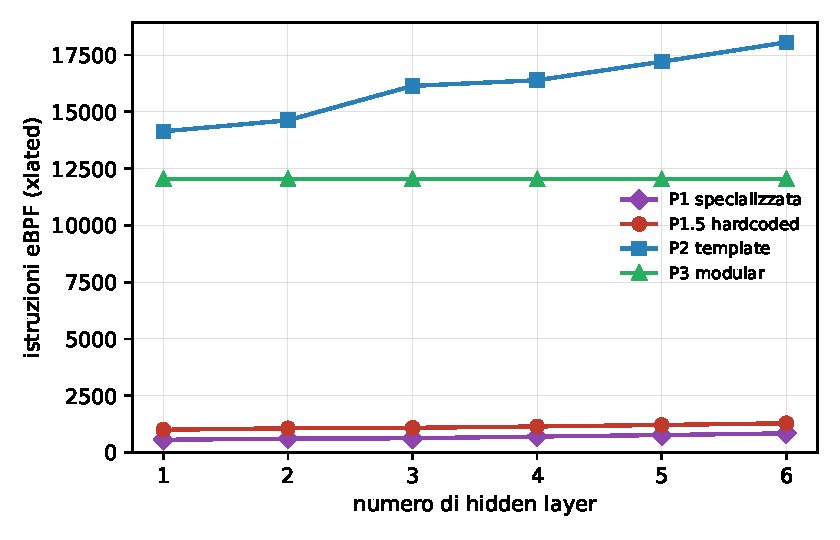
\includegraphics[width=0.92\textwidth]{../result/scaling_depth_insns.pdf}
\end{center}

\begin{lezione}
\textbf{P2 cresce di circa 780 istruzioni per ogni hidden layer. P3 di zero.}
\end{lezione}

P3 srotola \emph{un} solo strato denso generico e ci rientra a ogni passo della
rete, quindi la profondità non entra nel programma: la sua riga è
perfettamente orizzontale, da uno a sei strati. P2 deve srotolarli tutti,
perché è un programma solo.

Ma la storia non finisce lì:

\begin{center}
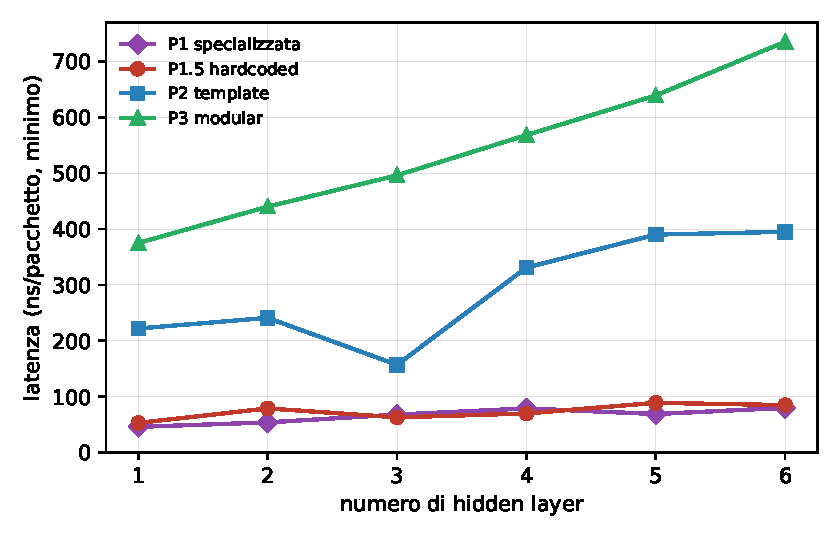
\includegraphics[width=0.92\textwidth]{../result/scaling_depth_latenza.pdf}
\end{center}

\begin{lezione}
\textbf{E P3 lo paga in tempo: circa 70 nanosecondi per strato}, contro i 36 di
P2. Sono i salti fra programmi, da 2 a 7.
\end{lezione}

Le due figure hanno la \emph{stessa} causa vista dai due lati. P3 è più piccolo
\textbf{perché} riusa un pezzo, ed è più lento \textbf{perché} riusarlo costa
un salto e delle letture ogni volta. È il compromesso della modularità, ridotto
a due numeri.

\section{Aggiornare il modello: due ordini di grandezza}

\begin{center}
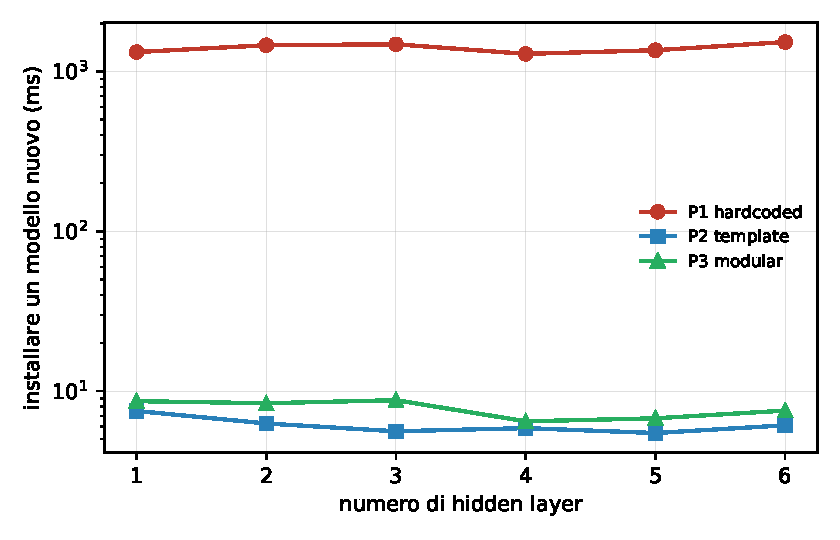
\includegraphics[width=0.92\textwidth]{../result/scaling_depth_update.pdf}
\end{center}

Attenzione alla scala verticale: è \textbf{logaritmica}. Su scala lineare le due
curve basse sarebbero schiacciate sullo zero e si vedrebbe una curva sola.

\begin{lezione}
Installare un modello nuovo su un nodo già in servizio costa \textbf{circa 1,4
secondi} in P1 --- che deve rigenerare il C e richiamare il compilatore --- e
\textbf{circa 7 millisecondi} in P2 e P3, che scrivono in una tabella.

È la misura che decide se una pipeline è usabile in una rete che cambia.
\end{lezione}

\section{Congelare il nodo: conviene?}

L'indice del nodo è una \textbf{costante del deployment}: un nodo non cambia di
posto. Il codice però lo legge a runtime, e per farlo porta uno switch con un
caso per ogni nodo della rete --- 52 casi per Germany50, di cui ne esegue
\emph{uno}.

Congelandolo a tempo di generazione lo switch sparisce, e con lui la lettura
della tabella. Restano quattro numeri costanti, che il compilatore può piegare
dentro al conto.

\begin{center}
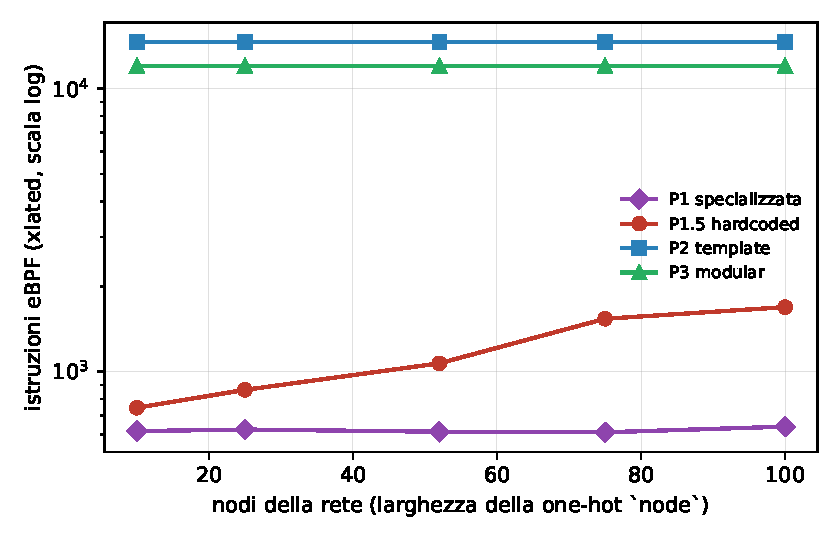
\includegraphics[width=0.92\textwidth]{../result/scaling_nodes_insns_log.pdf}
\end{center}

\begin{lezione}
La taglia della rete entra nel programma \textbf{solo} nella P1.5, che passa da
746 a 1\,692 istruzioni fra 10 e 100 nodi.

Congelando il nodo quella dipendenza \textbf{sparisce}: la riga viola è piatta,
fra 611 e 640 a qualunque taglia.
\end{lezione}

(La scala è logaritmica: in lineare le due righe P1 resterebbero schiacciate
contro le quattordicimila di P2, e il confronto fra loro --- che è il punto della
figura --- non si vedrebbe.)

\subsection*{Ma la velocità non cambia}

\begin{center}
\small
\begin{tabular}{@{}lrrrrr@{}}
\toprule
\textbf{nodi} & 10 & 25 & 52 & 75 & 100 \\
\midrule
P1 specializzata & 58 & 68 & 54 & 55 & 55 ns \\
P1.5 hardcoded   & 61 & 60 & 57 & 59 & 61 ns \\
\bottomrule
\end{tabular}
\end{center}

Praticamente identiche, dentro il rumore.

\begin{lezione}
Il motivo per cui la \emph{dimensione} crolla e il \emph{tempo} no è lo stesso:
lo switch ha 52 casi ma ne esegue uno. A runtime è un salto indicizzato, che
costa poco; quelle 208 assegnazioni sono compilate per eseguirne quattro.

Toglierle libera molto \textbf{spazio} e quasi nessun \textbf{tempo}.
\end{lezione}

\subsection*{Il controllo, e perché ci si può fidare}

Come si fa a essere sicuri che il divario venga davvero dalla one-hot del nodo e
non da qualcos'altro che è cambiato per caso? Si prende un vettore d'ingresso che
la feature \emph{non} la contiene:

\begin{center}
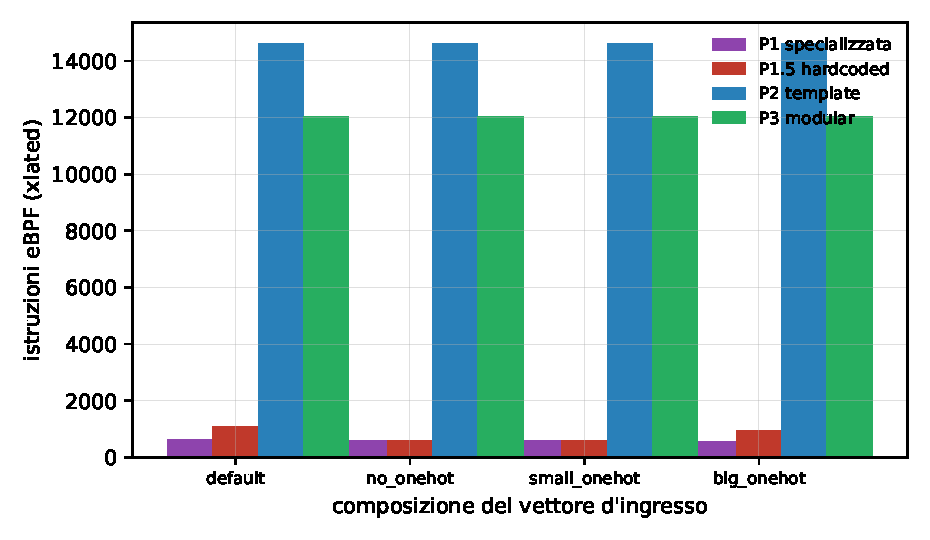
\includegraphics[width=0.92\textwidth]{../result/scaling_descriptor_insns.pdf}
\end{center}

Nelle due composizioni senza la feature \texttt{node} le due P1 sono
\textbf{identiche alla cifra} (599 e 599; 575 e 575). In quelle che ce l'hanno,
divergono. Il divario è tutto lì e nient'altro.

C'è poi una verifica che viene prima di ogni numero. Congelare il nodo significa
scegliere \emph{una colonna} della matrice dei pesi al momento di generare il
codice: sceglierne una sbagliata darebbe un programma più piccolo, più veloce, e
che calcola \textbf{un altro modello} --- e nessuna misura di costo se ne
accorgerebbe. Ottanta casi, dieci valori di TTL per otto configurazioni di link:
la versione congelata decide sempre la stessa classe di quella che legge il nodo
dalla tabella.

\subsection*{I due vantaggi non si sommano}

\begin{center}
\small
\begin{tabular}{@{}lrrrrr@{}}
\toprule
\textbf{pesi a zero} & 0\%\ & 25\%\ & 50\%\ & 75\%\ & 90\%\ \\
\midrule
P1 specializzata & 614 & 566 & 417 & 294 & \textbf{216} \\
P1.5 hardcoded   & 1\,071 & 939 & 686 & 363 & \textbf{224} \\
\bottomrule
\end{tabular}
\end{center}

Al 90\%\ di zeri il divario è sparito. Sparsità e nodo congelato sono \textbf{due
strade alla stessa riduzione}: se i pesi sono già quasi tutti zero, il
compilatore cancella lo switch da solo e non resta niente da congelare.

\subsection*{Il verdetto}

\begin{lezione}
Congelare il nodo \textbf{non è un'ottimizzazione di velocità}. È ciò che rende la
pipeline hardcoded \emph{praticabile su una rete grande}.

Lo switch della P1.5 cresce col numero di nodi moltiplicato per la larghezza del
primo strato. Su una topologia da 500 nodi con 8 neuroni sarebbero quattromila
assegnazioni srotolate, e c'è una taglia oltre la quale quel programma non si
carica più. La specializzata non ci arriva mai.

Il prezzo è \textbf{un binario per nodo}: 52 compilazioni e 52 installazioni,
una per macchina. Il costo di aggiornamento si moltiplica proprio per la
grandezza da cui la specializzazione ha appena liberato la dimensione.
\end{lezione}

Su Germany50, dove la differenza è fra 614 e 1\,071 istruzioni a parità di
velocità, è una scelta legittima in entrambe le direzioni. Su una rete dieci
volte più grande non lo è più.

\section{Due larghezze, due risposte opposte}

Questa coppia di figure è il risultato che preferisco di tutta l'analisi, perché
la risposta non è quella che verrebbe da indovinare.

\begin{center}
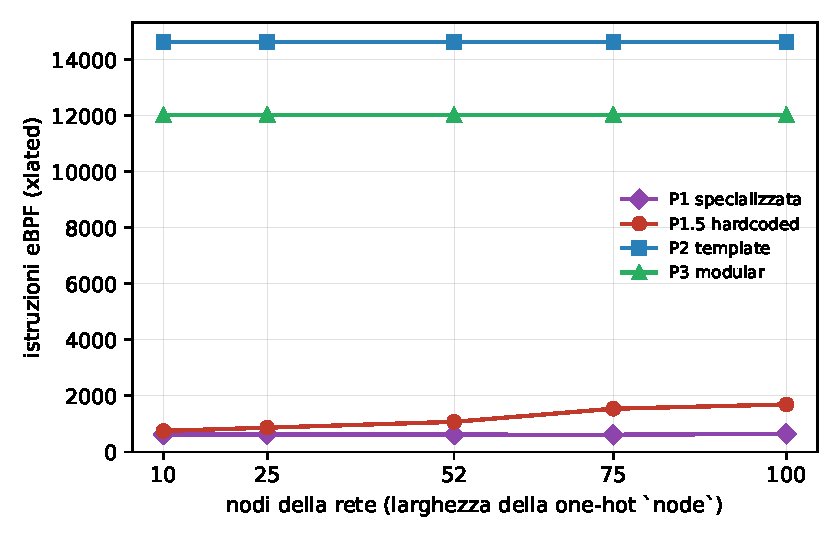
\includegraphics[width=0.92\textwidth]{../result/scaling_nodes_insns.pdf}
\end{center}

La taglia della \emph{rete} entra nel programma solo in P1, che passa da 746 a
1\,692 istruzioni fra 10 e 100 nodi: è lo switch della one-hot che si srotola.
P2 e P3 restano alla cifra esatta a ogni punto, perché il loro codice non
nomina mai la forma del modello.

E a runtime?

\begin{center}
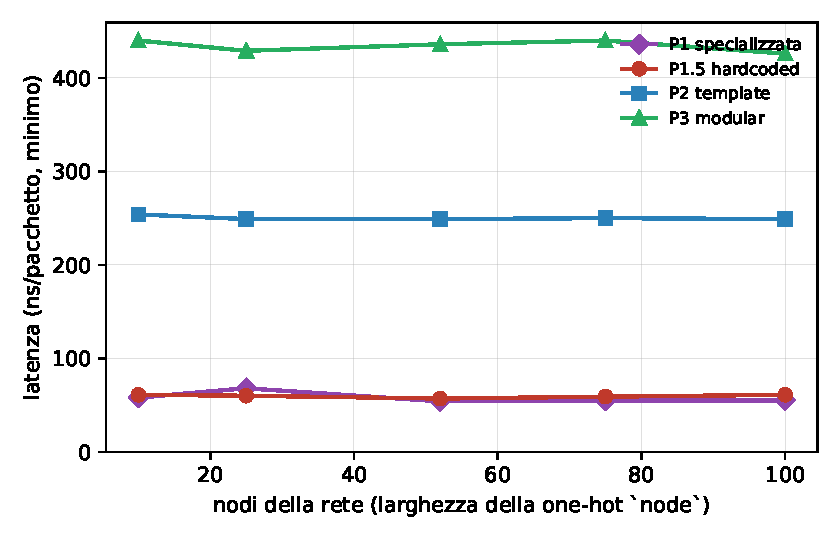
\includegraphics[width=0.92\textwidth]{../result/scaling_nodes_latenza.pdf}
\end{center}

\textbf{Piatte tutte e tre.} Cento nodi costano quanto dieci. Il motivo è
strutturale: una one-hot ha un solo uno, quindi il datapath legge \emph{una
sola colonna di pesi} qualunque sia la larghezza del vettore.

Allargare i layer \emph{nascosti}, invece:

\begin{center}
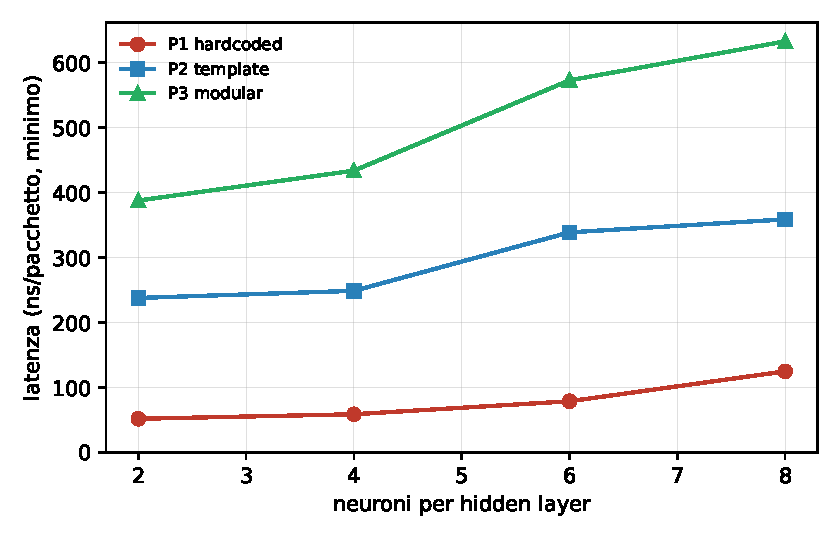
\includegraphics[width=0.92\textwidth]{../result/scaling_width_latenza.pdf}
\end{center}

\begin{lezione}
\textbf{La rete può crescere quanto vuole; il modello no.}

Allargare l'\emph{ingresso} è gratis a runtime, perché una one-hot legge una
colonna sola. Allargare i layer \emph{nascosti} si paga, su tutte e tre le
pipeline, perché ogni neurone in più sono pesi in più letti per ogni pacchetto.
\end{lezione}

\section{I pesi contano, ma solo per una delle tre}

\begin{center}
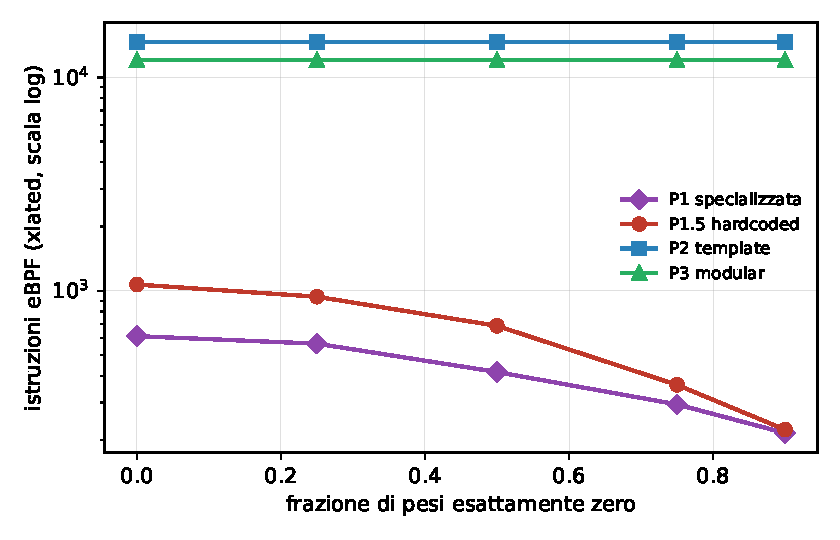
\includegraphics[width=0.92\textwidth]{../result/scaling_sparsity_insns_log.pdf}
\end{center}

Stessa identica forma in tutti e cinque i punti: cambia solo \emph{quanti} pesi
valgono zero.

\begin{lezione}
Con il 90\%\ dei pesi a zero, P1 passa da 1\,071 a \textbf{224 istruzioni}. P2 e
P3 non si muovono di una.
\end{lezione}

P1 scrive i pesi nel codice come numeri, quindi il compilatore vede una
moltiplicazione per zero e la cancella. Per P2 e P3 uno zero è un byte in una
tabella come un altro, e il programma è lo stesso.

Lo stesso vale per la composizione dell'ingresso: la figura del controllo, due
sezioni più su, mostra che cambiare \emph{quali} feature compongono il vettore
d'ingresso ricompila entrambe le P1, mentre P2 e P3 leggono il descrittore da
una tabella e non cambiano di una istruzione.

\section{Il risultato che non cercavamo}

Durante lo sweep una configurazione si è fatta rifiutare dal verificatore:
quattro hidden layer da quattro neuroni. Le forme intorno caricavano tutte,
inclusa quella \emph{più grande} con cinque strati. Nessuna proprietà della
profondità può produrre una cosa del genere.

Tenendo ferma la forma e cambiando solo il seme casuale dei pesi:

\begin{center}
\small
\begin{tabular}{@{}rl@{}}
\toprule
\textbf{seme} & \textbf{esito} \\
\midrule
42  & \textcolor{bad}{\textbf{rifiutato}} \\
1   & carica, 1\,119 istruzioni \\
2   & carica, 1\,175 \\
7   & carica, 1\,118 \\
999 & carica, 1\,075 \\
\bottomrule
\end{tabular}
\end{center}

Il seme 1 carica a 1\,119 istruzioni; il 42 viene rifiutato a 1\,120. Una
istruzione di differenza.

\begin{lezione}
\textbf{In P1, riaddestrare un modello senza toccare l'architettura può renderlo
non caricabile.} Stessa rete, stessi iperparametri, pesi nuovi, e il nodo lo
rifiuta.

P2 e P3 non hanno questo rischio: per loro i pesi sono byte in una tabella, e
che il programma si carichi dipende solo dalla forma.
\end{lezione}

È il rovescio esatto del vantaggio di due pagine fa. La stessa riduzione del
compilatore che porta P1 a 224 istruzioni è quella che lo rende imprevedibile.
Un compromesso vero, misurato su entrambi i lati.

Il meccanismo preciso --- \emph{quale} limite del kernel --- non è stato
confermato, e non va inventato: il messaggio d'errore parla di un programma
troppo lungo e cita un limite di 4096 istruzioni che nella stessa esecuzione P2
supera di quattro volte. È la stessa costante morta già incontrata sul capitolo
del verificatore.

\section{Che cosa questi grafici non dicono}

\begin{itemize}
\item \textbf{Non si confrontano latenze prese da assi diversi.} A programma
      identico, P2 misura circa 250 ns su due assi e circa 310 sugli altri due:
      la macchina si è caricata a metà esecuzione. Dentro un asse i confronti
      reggono. Le istruzioni, che sono deterministiche, si confrontano ovunque.
\item La figura sulla larghezza va letta per la \emph{direzione}, non per la
      pendenza, per lo stesso motivo.
\item Oltre circa 115 nodi non si va senza alzare un tetto compilato e
      \textbf{rimisurare}.
\end{itemize}

% ==================================================================
\chapter{Quel che resta}

\section{Fatto}

\begin{itemize}
\item semantica delle classi dichiarata, mai dedotta; catena classe $\to$ azione
      $\to$ porta logica $\to$ interfaccia;
\item motore indipendente dallo scenario, dimostrato su cinque topologie diverse;
\item emulatore rimosso; verifica end-to-end su datapath reale con XDP native;
\item errore del bias nell'ultimo strato corretto;
\item feature dell'interfaccia d'ingresso resa viva in tutte e tre le pipeline;
\item \textbf{indice del nodo} letto a runtime da tabella in tutte e tre: era
      l'ultimo ingresso su cui le pipeline non concordavano, e pesa 208 pesi su
      319;
\item primo strato riscritto con i cicli invertiti in P2 e P3: stesso risultato
      bit per bit, un terzo dei rami in meno, e il margine di verifica che ne è
      uscito ha permesso di \textbf{recuperare il tetto sulle code} (da 1 a 8) e
      di \textbf{rimettere la riga delle letture di tabella}, che era n.d.;
\item oggetto precompilato (AOT) compilato, caricato e misurato: aggiornamento
      del modello da 1\,242 ms a 37 ms, a parità di costo per pacchetto;
\item tabella dei risultati rifatta su uno stato del codice solo;
\item \textbf{analisi parametrica} su cinque assi e tre pipeline: le pendenze
      sono diverse, ed è la misura che giustifica l'esistenza di tre pipeline
      invece di una;
\item \textbf{versione P1 specializzata}: congela anche l'indice del nodo, e
      toglie alla pipeline hardcoded la dipendenza dalla taglia della rete ---
      al prezzo di un binario per nodo;
\item P2 non è più fissa a due hidden layer: la profondità è diventata un
      inviluppo compilato come già lo erano le larghezze --- al prezzo, onesto e
      misurato, di una ricompilazione per profondità.
\end{itemize}

\section{Aperto}

\begin{itemize}
\item \textbf{Throughput reale}: generare traffico a ritmo e misurare pacchetti
      al secondo, perdite e carico di CPU. È la misura che manca se la metrica
      principale è la velocità.
\item \textbf{Versione intermedia fra P1 e P2}: pesi scritti nel codice ma
      descrittore letto a runtime. Oggi il salto fra P1 e P2 confonde due
      cambiamenti insieme, e non si può attribuire il costo all'uno o all'altro.
\item \textbf{Hardware vero}: la scheda di rete di questa macchina virtuale è
      emulata e non supporta XDP native. I numeri assoluti restano non citabili
      come prestazioni di sistema.
\item \textbf{Il tetto sull'uscita di P2}: lo strato finale è srotolato a 32
      classi per un modello che ne ha 7, cioè 256 moltiplicazioni dove ne
      servono 28. Abbassarlo ridurrebbe molto il programma, ma \emph{cambia il
      comportamento}: restringe l'insieme dei modelli rappresentabili. La strada
      pulita è generare quel tetto dall'inviluppo dichiarato dal deployment
      invece di fissarlo nel sorgente --- una ricompilazione per inviluppo, non
      per modello.
\item \textbf{I salti fra programmi di P3}: sono tre per pacchetto ed è lì che
      sta la latenza, non nella dimensione. Ridurli è un lavoro diverso da
      quello fatto finora.
\item \textbf{Perché quel modello non si carica}: sappiamo che dipende dai pesi
      e non dall'architettura, ma non \emph{quale} limite del kernel venga
      toccato. Il messaggio d'errore ne nomina uno sbagliato. Serve il registro
      del verificatore, ed è un'ora di lavoro, non una settimana.
\item \textbf{Rimisurare a macchina scarica}: metà delle latenze dell'analisi
      parametrica sono state prese mentre la VM era occupata. Le istruzioni no,
      quelle sono deterministiche.
\end{itemize}

\section{Il filo conduttore}

Guardando indietro, quasi tutti i problemi trovati a settembre hanno la stessa
forma. Non erano calcoli sbagliati: erano \textbf{assunzioni non dichiarate} che
risultavano vere per caso nell'unica configurazione mai provata.

\begin{center}
\small
\begin{tabular}{@{}ll@{}}
\toprule
\textbf{Assunzione} & \textbf{Vera solo perché} \\
\midrule
classe $k$ $=$ interfaccia $k$ & le porte erano numerate come le classi \\
DROP $=$ ultima classe & nel modello depositato capitava così \\
$n_{\text{nodi}} = 52$ di default & si provava una topologia sola \\
\texttt{eth0} $=$ ifindex 2 & si provava dentro un container pulito \\
bias dell'uscita $\times\, s^0$ & si provava coi link tutti attivi \\
one-hot del nodo $=$ \texttt{model\_id} & si registrava un modello solo \\
tabella vuota $=$ nodo 0 & l'array è preallocato a zero \\
si carica $\Rightarrow$ dipende dall'architettura & non si era mai cambiato solo i pesi \\
\bottomrule
\end{tabular}
\end{center}

E quasi tutte sono emerse allo stesso modo: cambiando \emph{una} condizione che
nessun test aveva mai cambiato.

\begin{lezione}
Un test verde dice che il codice si comporta come il test si aspetta. Non dice
che il test stia chiedendo qualcosa.
\end{lezione}

\end{document}
